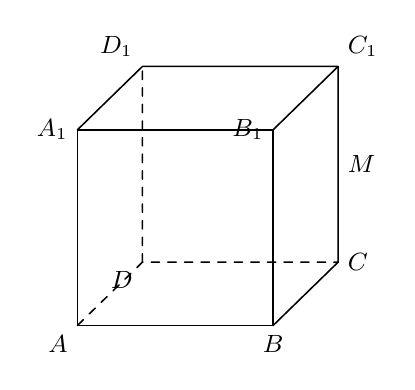
\begin{tikzpicture}[scale=.70, every node/.style={font=\small}, line cap=round, line join=round]
  \coordinate (A)  at (0,0);
  \coordinate (B)  at (3.55,0);
  \coordinate (B1) at (3.55,3.55);
  \coordinate (A1) at (0,3.55);
  \coordinate (D)  at (1.18,1.15);
  \coordinate (C)  at (4.73,1.15);
  \coordinate (C1) at (4.73,4.70);
  \coordinate (D1) at (1.18,4.70);
  \coordinate (M)  at (4.73,2.925);

  \draw[line width=.56pt] (A)--(B)--(B1)--(A1)--cycle;
  \draw[line width=.56pt] (A1)--(D1)--(C1)--(B1);
  \draw[line width=.56pt] (B)--(C)--(C1);
  \draw[dashed, line width=.56pt] (A)--(D)--(C) (D)--(D1);

  \node[below left] at (A) {$A$};
  \node[below] at (B) {$B$};
  \node[right] at (C) {$C$};
  \node[below left] at (D) {$D$};
  \node[left] at (A1) {$A_1$};
  \node[left] at (B1) {$B_1$};
  \node[above left] at (D1) {$D_1$};
  \node[above right] at (C1) {$C_1$};
  \node[right] at (M) {$M$};
\end{tikzpicture}
